% =============================================================================
%  Brick and the Mixture-of-Models (MoM) Paradigm
%  Bridging Open- and Closed-Weight LLM Pools
%  Author: Francesco Massa (Seeweb), May 2026
%  Style: article + twocolumn standard. Black titles. Blue only for hyperlinks.
%  No em dashes anywhere.
% =============================================================================
\documentclass[twocolumn,10pt,a4paper]{article}

% ---- Fonts (Adobe Source family) -------------------------------------------
\usepackage[T1]{fontenc}
\usepackage[utf8]{inputenc}
\usepackage[english]{babel}
\usepackage[default]{sourceserifpro}
\usepackage[scaled=0.93]{sourcesanspro}
\usepackage[scaled=0.85]{sourcecodepro}

% ---- Geometry --------------------------------------------------------------
\usepackage[margin=2cm,top=2cm,bottom=2cm,columnsep=18pt]{geometry}

% ---- Typography ------------------------------------------------------------
\usepackage{microtype}
\setlength{\parindent}{0pt}
\setlength{\parskip}{3pt}

% ---- Colors (blue is for hyperlinks ONLY) ---------------------------------
\usepackage{xcolor}
\definecolor{linkblue}{HTML}{1F4E79}

% ---- Black section headings with thin gray underline ----------------------
\usepackage{titlesec}
\titleformat{\section}
  {\normalfont\large\bfseries\sffamily}{\thesection.}{0.5em}{\MakeUppercase}
  [\vspace{1pt}\titlerule]
\titleformat{\subsection}
  {\normalfont\normalsize\bfseries\sffamily}{\thesubsection.}{0.5em}{}
\titlespacing*{\section}{0pt}{1.2em}{0.5em}
\titlespacing*{\subsection}{0pt}{0.7em}{0.3em}

% ---- Tables, figures, captions --------------------------------------------
\usepackage{graphicx}
\usepackage{booktabs}
\usepackage{multirow}
\usepackage{array}
\usepackage{tabularx}
\usepackage{float}
\usepackage[font=small,labelfont=bf,labelsep=period,skip=4pt]{caption}
\renewcommand{\arraystretch}{1.18}

% ---- Math + URLs + hyperref -----------------------------------------------
\usepackage{amsmath,amssymb}
\usepackage{url}
\usepackage{hyperref}
\usepackage{fontawesome5}
\usepackage{enumitem}
\usepackage{tikz}
\usetikzlibrary{positioning,arrows.meta,calc,fit,backgrounds}
\usepackage{placeins}
\hypersetup{colorlinks=true,linkcolor=linkblue,urlcolor=linkblue,citecolor=linkblue}

\graphicspath{{figures/}}
\pagestyle{plain}

% Inline mini-logo helper for tables ("\mdlogo{qwen}" => 1em-high logo).
\newcommand{\mdlogo}[1]{\raisebox{-.3ex}{\includegraphics[height=1.05em]{logos/#1_logo}}}

% ---- Title block reused inside two-column abstract wrap -------------------
\newcommand{\customheader}{%
  \noindent
  \hfill{\sffamily\small\color{black!65}Technical Report \textbullet{} May 2026 \textbullet{} v0.1}\par
  \vspace{4pt}{\color{black!40}\hrule height 0.6pt}%
}

\title{}\author{}\date{}

\begin{document}
\thispagestyle{empty}

% =============================================================================
%  Full-width title + abstract band (single column on page 1)
% =============================================================================
\twocolumn[%
  \begin{@twocolumnfalse}%
    \vspace{12pt}
    \begin{center}
      {\Huge\bfseries Brick and the Mixture-of-Models (MoM) Paradigm}\par
      \vspace{4pt}
      {\Large\color{black!75} Bridging Open- and Closed-Weight LLM Pools}\par
      \vspace{14pt}
      {\Large\bfseries
        \raisebox{-3pt}{
\includegraphics[height=16pt]{logos/seeweb_logo.png}}\, \href{https://seeweb.it/en}{Seeweb}
        \quad
        \raisebox{-3pt}{
\includegraphics[height=16pt]{logos/regolo_logo.jpg}}\, \href{https://regolo.ai}{Regolo.ai}
        \quad\textbullet\quad May 2026}\par
      \vspace{12pt}
      \begin{tabular}{c@{\hspace{3em}}c}
        {\large Francesco Massa} & {\large Marco Cristofanilli} \tabularnewline
        {\small \href{mailto:f.massa@regolo.ai}{f.massa@regolo.ai}} &
        {\small \href{mailto:marco.c@seeweb.it}{marco.c@seeweb.it}} \tabularnewline
      \end{tabular}\par
      \vspace{8pt}
      {\normalsize \raisebox{-2.5pt}{\large\faGithub}\, \href{https://github.com/regolo-ai/brick-SR1}{regolo-ai/brick-SR1} \quad\textbullet\quad \raisebox{-2.5pt}{
\includegraphics[height=12pt]{figures/logos/hf_logo.png}}\, \href{https://huggingface.co/regolo}{huggingface.co/regolo}}
    \end{center}
    \vspace{12pt}

    {\color{black!50}\hrule height 0.4pt}\vspace{4pt}
    {\noindent\bfseries Abstract.}\space
    What is difficult for a language model? Defining difficulty is one of the hardest problems in deployment engineering, and the only reliable answer is empirical. Once correctness is measured per query and per model, the question becomes: can a router dispatch each query to the cheapest model that will answer it correctly?

    \medskip\noindent Existing systems route on surface features: domain labels, keywords, token count. We call this \emph{superficial routing}. It collapses the within-domain variance that actually determines which model succeeds, since a one-line question can target an unsolved problem while a long boilerplate prompt can wrap a trivial task.

    \medskip\noindent This paper takes a further step toward the \emph{Mixture of Models} (MoM) paradigm, where an external router dispatches each query to the cheapest full model in a heterogeneous pool. We present \textbf{Brick}, a multimodal router that scores each model on six capability dimensions and combines this with a per-query difficulty estimate to produce a cost-penalized score. A continuous preference knob $r$ lets operators slide between a \emph{max-quality} profile and a \emph{max-saving} profile, turning the quality-versus-spend trade-off into a deploy-time parameter rather than a code change. On \textbf{Dataset A} ($5{,}504$ queries, $\kappa{=}0.761$), Brick at max-quality reaches $\mathbf{76.98\%}$ accuracy, beating the best single model (\texttt{kimi2.6}, $75.02\%$) and all external routers (RouteLLM, FrugalGPT, Cascade Routing); at max-saving it cuts average cost per query by $4\times$ against always-\texttt{kimi} while staying within $3$\,pp of its accuracy. At production scale, even small per-request savings compound across millions of calls, making the knob a direct cloud-bill lever. Median end-to-end latency is $22.8$\,s vs $51.2$\,s for always-\texttt{kimi}; the three-model oracle bound is $83.25\%$.

    \par\vspace{4pt}
    {\noindent\bfseries Keywords.}\space LLM routing, mixture of models, capability classification, cost-aware inference, open-weight models.
    \vspace{4pt}{\color{black!50}\hrule height 0.4pt}\vspace{12pt}
  \end{@twocolumnfalse}%
]

% =============================================================================
\section{Introduction}\label{sec:intro}
% =============================================================================
Identifying what is \emph{difficult} for a given language model is one of the harder skills a deployment engineer can develop. Training data, architecture changes, and reinforcement post-training all interact in opaque ways, so deciding which model is best for a task is in practice an empirical exercise: only repeated evaluation reveals where a model excels and where it fails silently.

A growing collection of public evaluation suites makes this exercise tractable. Once response correctness can be measured per query and per model, the question becomes: given a pool of $K$ candidate models with heterogeneous price and capability profiles, can a router send each query to the cheapest model that will answer it correctly? This is the routing problem we address. Two engineering constraints make it non-trivial. First, capability is multi-dimensional; a single model can be strong at code while weak at planning, so global ranking is misleading. Second, both cost and latency vary across models by an order of magnitude, so the wrong choice penalizes either accuracy or the bill.

This paper contributes:
\begin{enumerate}[noitemsep,topsep=3pt,leftmargin=1.4em,label=\arabic*.]
  \item The \emph{Mixture-of-Models} (MoM) paradigm as a deployment framing for routing across heterogeneous full-weight models including mixed open-weight and commercial pools (§\ref{sec:mom}).
  \item A critique of two superficial routing strategies that fail to capture intra-domain difficulty (§\ref{sec:superficial}).
  \item \textbf{Brick}, a calibrated MoM router with an explicit capability vector representation and a user-facing preference knob (§\ref{sec:brick}).
  \item Experimental results on Dataset A showing Brick exceeds the best single-model baseline at a fraction of its perceived latency (§\ref{sec:results}, §\ref{sec:latency}).
\end{enumerate}

\section{The Mixture-of-Models (MoM) Paradigm}\label{sec:mom}
Training a new frontier model from scratch costs tens of millions of dollars and months of compute. A simpler question is: why not use the models already available? The market offers a wide range of pretrained models at different price points and capability profiles. Rather than collapsing this diversity into a single choice, we decided to build a custom architecture on top of it. We call this the \emph{Mixture of Models} (MoM) paradigm: a pool of whole pretrained models, dispatched one per query through an external router. The unit of routing is a model, not a layer. MoM differs from \emph{Mixture of Experts} (MoE), where sparse sub-networks inside a single model are activated per token; here the mixing happens at deployment time, across independent systems.

MoM is appealing for three operational reasons:

\begin{itemize}\setlength{\itemsep}{3pt}
  \item \textbf{Heterogeneous pricing.} Frontier commercial models charge ten to one hundred times what local open-weight models cost. A router that uses them only when needed makes the median query cheap without losing the long tail.
  \item \textbf{OW+CW bridging.} An MoM pool can mix open-weight models hosted in a controlled environment with closed-weight commercial APIs. The router lets an operator capture the data-locality and price benefits of open weights on easy queries while reserving expensive closed-weight calls for hard ones.
  \item \textbf{Capability complementarity.} Models from different vendors and training recipes often have complementary error sets. As shown in §\ref{sec:dataset}, the three-model oracle on Dataset A reaches $83.25\%$, well above any single model.
\end{itemize}

The rest of this paper takes Brick as a concrete instantiation of MoM. The geometric routing rule and the calibration procedure are properties of Brick, not of the MoM paradigm itself; alternative MoM realizations are possible and are discussed in §\ref{sec:discussion}.

\section{Limitations of Superficial Routing}\label{sec:superficial}
Two routing strategies recur in production systems and deserve to be ruled out before introducing Brick.

\textbf{Domain-based routing} maps the query to a coarse domain (science, math, humanities, code) and dispatches to a per-domain best model. The hidden assumption is that, conditional on the domain, models rank uniformly. This assumption fails because difficulty varies sharply inside a domain: a request to write a Python calculator and a request to solve a Riemann-zeta question are both ``code'' or both ``math'' depending on framing, but require different models. Domain-based routing collapses this variance and over-pays on easy queries.

\textbf{Length- and keyword-based routing} maps the query to a complexity score from token count and regex hits. The assumption is that long or jargon-rich queries are hard, and short queries are easy. This also fails: a one-line question may target an unsolved problem, while a long boilerplate prompt may wrap a trivial transformation. Token count is a poor proxy for required capability.

The remainder of this paper treats routing as a decision in capability space, not in surface-feature space.

\section{Model Pool}\label{sec:pool}
We use a fixed three-model pool:
\[
  \mathcal{M} =
  \{\texttt{qwen3.5-9b},\ \texttt{deepseek-v4-flash},\ \texttt{kimi2.6}\}.
\]
The pool spans three quality-and-cost regimes: \texttt{qwen3.5-9b} as a state-of-the-art under-$10$B-parameter open-weight model, \texttt{deepseek-v4-flash} as a state-of-the-art under-$500$B open-weight model, and \texttt{kimi2.6} as a frontier open-source contender. Per-call normalized costs used in the routing math are
\[
  a_{\text{qwen}}{=}0.10,\quad a_{\text{ds4}}{=}0.40,\quad a_{\text{kimi}}{=}0.60.
\]
These dimensionless ratios are calibrated to public per-token pricing at the time of evaluation. They preserve the relative cost gap rather than committing to absolute USD values that drift between vendors.
Formally, given the public output price $p_m$ in USD per $10^6$ tokens, the cost scalar is
\[
  a_m = \frac{p_m}{p_{\mathrm{ref}}}, \qquad p_{\mathrm{ref}} = 1.00\ \text{USD}/10^6\ \text{tokens}.
\]
At evaluation time (May 2026) the reference prices were $p_{\text{qwen}}{=}0.10$, $p_{\text{ds4}}{=}0.40$, $p_{\text{kimi}}{=}0.60$ USD per $10^6$ output tokens, yielding the values above directly. The scalar $a_m$ is locked into the Brick configuration at calibration time and is not updated at inference.

\section{Dataset A}\label{sec:dataset}
Brick is evaluated on Dataset~A, a stratified routing-evaluation benchmark of $N{=}5{,}504$ queries covering six capability dimensions. Table~\ref{tab:composition} summarizes the per-source composition. The corpus is built from fourteen license-clean upstream sources and three custom curated subsets. Each row carries a deterministic identifier, a typed evaluation payload, pre-computed token counts under the three target tokenizers, and a license tag enabling compliant redistribution.

\begin{table*}[!t]
\centering
\small
\caption{Per-source composition of Dataset~A ($N{=}5{,}504$). Counts may differ from the original release ($N{=}5{,}339$) due to the addition of $165$ planning multi-turn rows in revision $v0.4$.}
\label{tab:composition}
\begin{tabular}{l l r l}
\toprule
\textbf{Dimension} & \textbf{Source} & \textbf{Count} & \textbf{License} \\
\midrule
\multirow{2}{*}{instruction\_following}
  & IFEval~\cite{zhou2023ifeval}                & 541       & apache-2.0     \\
  & IFBench~\cite{pyatkin2025ifbench}           & 300       & ODC-BY-1.0     \\
\midrule
coding
  & LiveCodeBench-v6~\cite{jain2024livecodebench} & $1{,}000$ & cc-by-4.0      \\
\midrule
\multirow{3}{*}{math\_reasoning}
  & MATH-500~\cite{hendrycks2021math}            & 500       & mit            \\
  & AIME-2025                                    & 30        & qwen-derived   \\
  & GSM8K~\cite{cobbe2021gsm8k}                  & 470       & mit            \\
\midrule
\multirow{3}{*}{world\_knowledge}
  & SimpleQA~\cite{wei2024simpleqa}              & 700       & mit            \\
  & MMLU-Pro-Humanities~\cite{wang2024mmlupro}   & 102       & mit            \\
  & GPQA-Diamond~\cite{rein2024gpqa}             & 0 (gated) & cc-by-4.0      \\
\midrule
\multirow{3}{*}{creative\_synthesis}
  & EQ-Bench-Creative-v3~\cite{paech2024eqbench} & 96        & EQ-Bench terms \\
  & LitBench~\cite{stanford2025litbench}         & 500       & qwen-derived   \\
  & Custom-Validated                             & 100       & qwen-derived   \\
\midrule
\multirow{3}{*}{planning\_agentic}
  & BFCL-v4~\cite{yan2024bfcl}                   & 500       & apache-2.0     \\
  & tau-bench~\cite{yao2024taubench}             & 165       & mit            \\
  & Planning-Custom (incl. multi-turn)           & 500       & qwen-derived   \\
\midrule
\multicolumn{2}{l}{\textbf{Total}} & $\mathbf{5{,}504}$ & \\
\bottomrule
\end{tabular}
\end{table*}

\subsection{Quality validation and oracle bound}
The construction pipeline is validated in three tiers: deterministic schema and length checks, LLM-as-judge calibration against an audited reference subset, and a dual-reviewer manual audit on $n{=}102$ stratified samples. The manual audit yields Cohen's $\kappa{=}0.761$ on a 4-class rubric and $\kappa{=}0.951$ on the binary collapse, both above the conventional substantial-agreement threshold.

Aggregate per-model response accuracy on Dataset~A is reported in Table~\ref{tab:standalone_response_accuracy}, together with the achievable three-model oracle bound. A query is counted as solved if the model's response passes the per-protocol grader. The oracle counts a query as solved if any of the three models would have solved it; the residual $922$ queries are unsolvable by the current pool.

\begin{table}[H]
\centering
\caption{Standalone per-model response accuracy and three-model oracle bound on Dataset~A.}
\label{tab:standalone_response_accuracy}
\small
\begin{tabular}{l r r}
\toprule
\textbf{System} & \textbf{Solved} & \textbf{Accuracy} \\
\midrule
always \mdlogo{qwen}\,\texttt{qwen}    & $3{,}477 / 5{,}504$ & $63.17\%$ \\
always \mdlogo{ds4}\,\texttt{ds4}      & $4{,}056 / 5{,}504$ & $73.69\%$ \\
always \mdlogo{kimi}\,\texttt{kimi}    & $4{,}129 / 5{,}504$ & $75.02\%$ \\
\midrule
three-model oracle      & $4{,}582 / 5{,}504$ & $\mathbf{83.25\%}$ \\
unsolvable (any model)  & $922 / 5{,}504$    & $16.75\%$ \\
\bottomrule
\end{tabular}
\end{table}

Notably, \texttt{kimi2.6} is not the per-query oracle: it fails $1{,}375$ queries, of which $453$ are correctly answered by at least one cheaper model. An oracle restricted to \texttt{kimi}$+$\texttt{ds4} reaches $81.96\%$, a gain of $6.94$ pp over \texttt{kimi} alone. This residual headroom is the upside an MoM router can in principle capture.

The dataset is publicly available at \href{https://huggingface.co/datasets/regolo/brick-dataset-A-routing-eval}{regolo/brick-dataset-A-routing-eval}.

\section{External Router Baselines}\label{sec:baselines}
We benchmark four published routing strategies on Dataset~A under the same three-model pool: RouteLLM in its binary and tournament variants~\cite{ong2024routellm}, FrugalGPT-style cascade routing~\cite{chen2023frugalgpt}, and Cascade Routing~\cite{jitkrittum2024cascade}. We use the public reference checkpoints in zero-shot mode; no fitting is performed on Dataset~A.

\begin{table*}[!t]
\centering
\caption{External router baselines on Dataset~A. Accuracy is response accuracy under the per-protocol grader. Distribution reports selected-model shares as percentages (qwen / ds4 / kimi).}
\label{tab:external_baselines}
\small
\begin{tabular}{l r r c}
\toprule
\textbf{Router} & \textbf{Accuracy} & \textbf{Avg.\,cost} & \textbf{Distribution q\,/\,ds4\,/\,kimi (\%)} \\
\midrule
RouteLLM binary      & $21.31\%$           & $0.999$ & $0.04 / 0 / 99.96$ \\
RouteLLM tournament  & $21.31\%$           & $0.999$ & $0.04 / 0 / 99.96$ \\
FrugalGPT cascade    & $63.17\%$           & $0.070$ & $100 / 0 / 0$ \\
Cascade Routing      & $28.96\%$           & $0.526$ & $18 / 61 / 21$ \\
always \mdlogo{qwen}\,qwen & $63.17\%$ & $0.100$ & $100 / 0 / 0$ \\
always \mdlogo{ds4}\,ds4   & $15.55\%$ & $0.500$ & $0 / 100 / 0$ \\
always \mdlogo{kimi}\,kimi & $21.28\%$ & $1.000$ & $0 / 0 / 100$ \\
\midrule
oracle               & $\mathbf{100.00\%}$ & $0.335$ & $63 / 16 / 21$ \\
\bottomrule
\end{tabular}
\end{table*}

Three observations are worth recording. First, RouteLLM, trained on a binary preference signal between two models, collapses on the three-model pool: it dispatches $99.96\%$ of queries to \texttt{kimi}, behaving as a noisy always-\texttt{kimi}. Second, FrugalGPT in cascade mode terminates at the cheapest model whenever its self-verification gates fire; in a three-model pool with cost ratio $1{:}4{:}6$, this collapses to always-\texttt{qwen} accuracy. Third, Cascade Routing routes to \texttt{ds4} on the majority of queries but does not match a tuned MoM router on aggregate accuracy.

The wider methodological observation is that cascade-style approaches commit to the cheapest model first and pay duplicate inference cost on rejection, which inflates perceived latency. Binary routers do not extend cleanly to $K{\ge}3$ pools without recursive pairing. Both classes are misaligned with MoM, which selects a single model per query in one decision step.

\section{Cost vs Performance Frontier}\label{sec:cost}
Figure~\ref{fig:cost_pareto} plots response accuracy against average normalized cost for the three single-model baselines, the four external routers, the five Brick preference profiles introduced in §\ref{sec:brick}, and the three-model oracle ceiling. Brick's max-quality profile dominates always-\texttt{kimi} on both axes: higher accuracy at lower cost. The Brick curve traces a Pareto front above the external routers across the operating range.

\begin{figure*}[!t]
\centering
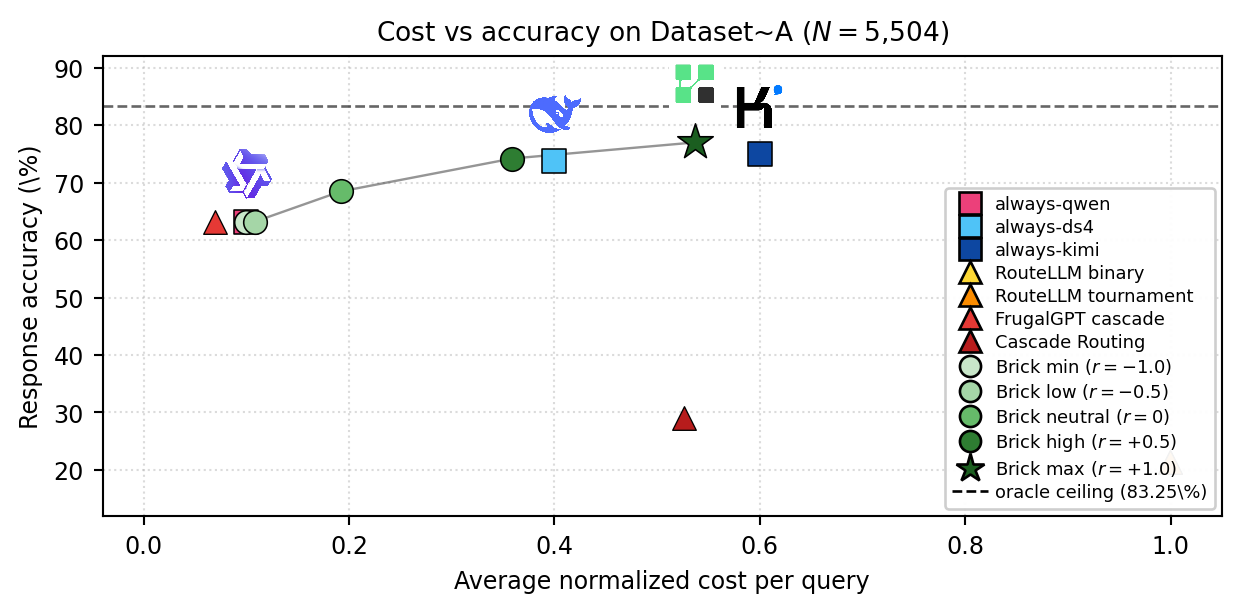
\includegraphics[width=\textwidth]{cost_pareto.png}
\caption{Cost vs response accuracy on Dataset~A. Single-model baselines are squares, external routers are triangles, Brick (MoM) profiles are circles (max profile is a star). The dashed line marks the three-model oracle ceiling.}
\label{fig:cost_pareto}
\end{figure*}

\section{Brick: A Calibrated MoM Router}\label{sec:brick}

\subsection{Pipeline}\label{sec:brick-pipeline}
\begin{samepage}
Brick processes each query through a deterministic six-step pipeline:
\nopagebreak
\begin{enumerate}\setlength{\itemsep}{3pt}\setlength{\parskip}{0pt}
  \item normalize and truncate the query text;
  \item match the query against high-precision keyword rules (e.g.\ explicit code fences) that can bias the capability distribution;
  \item compute a capability probability vector $p(x)\in\Delta^{D-1}$ (i.e.\ $p_c\!\ge\!0$ and $\sum_c p_c{=}1$) over a six-dimensional basis using a fine-tuned ModernBERT classifier;
  \item compute a complexity label and confidence using a separate complexity classifier, mapping to a base difficulty level $\tau_q$;
  \item compute a per-model capability score $J_m$ using the routing math of §\ref{sec:brick-math};
  \item select $m^{\star}=\arg\min_m J_m$ with deterministic tie-breaking.
\end{enumerate}
\end{samepage}

\begin{figure*}[!t]
\centering
% Brick architecture diagram (TikZ). Included via \input{} into paper.tex.
% Single-column tall vertical layout, Vaswani-style.
% Cartesian arrows only. Scorer decomposed into 5 sub-blocks + Cost Vector lateral.
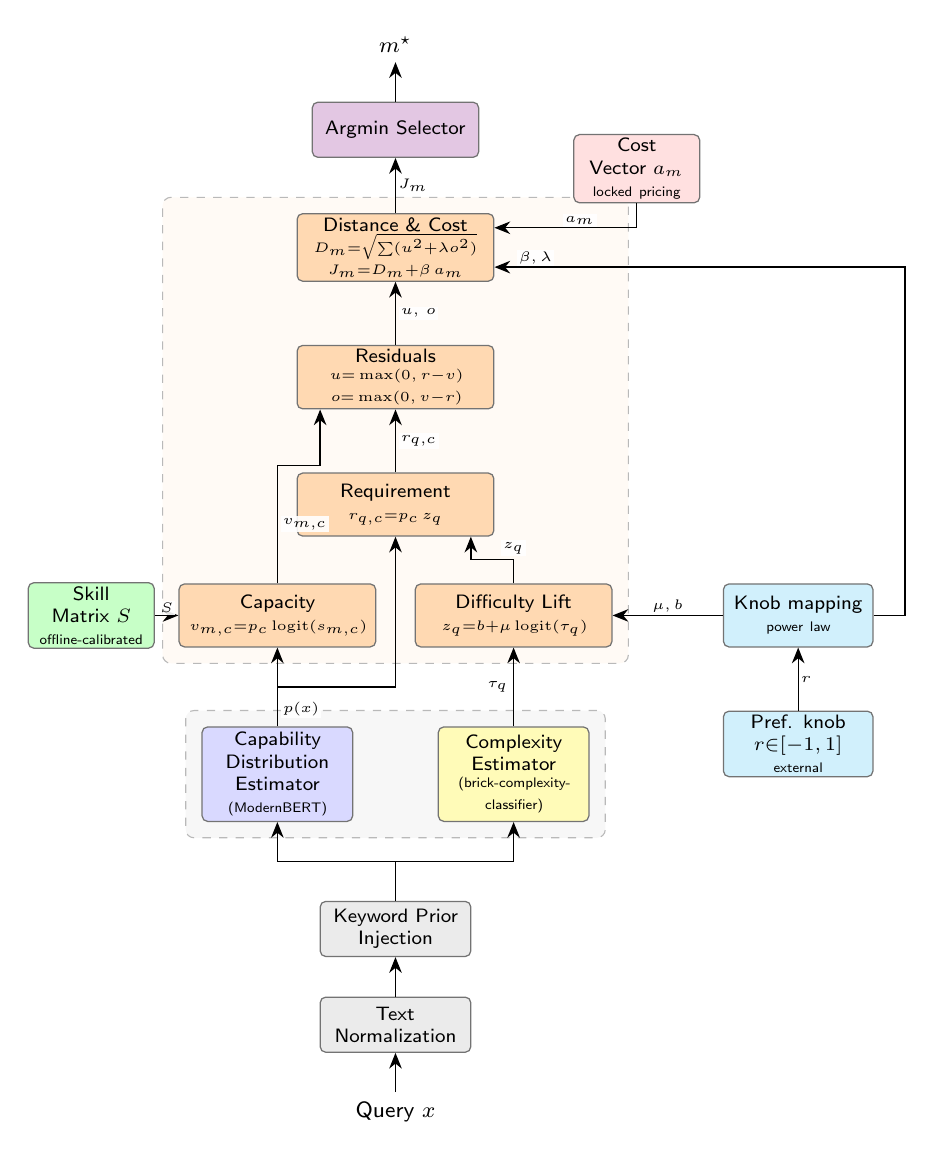
\begin{tikzpicture}[
    font=\sffamily,
    node distance=5mm and 5mm,
    box/.style    ={rectangle, rounded corners=2pt, draw=black!55,
                    line width=0.45pt, align=center, inner sep=1.6pt,
                    font=\sffamily\scriptsize, minimum height=7mm,
                    text width=18mm},
    norm/.style   ={box, fill=black!8},
    capbox/.style ={box, fill=blue!15,   text width=18mm, minimum height=12mm},
    cpx/.style    ={box, fill=yellow!28, text width=18mm, minimum height=12mm},
    sub/.style    ={box, fill=orange!30, text width=24mm, minimum height=8mm,
                    inner sep=1.4pt},
    skill/.style  ={box, fill=green!22,  text width=15mm, minimum height=8mm,
                    inner sep=1.4pt},
    cost/.style   ={box, fill=red!12,    text width=15mm, minimum height=8mm,
                    inner sep=1.4pt},
    knob/.style   ={box, fill=cyan!18,   text width=18mm, minimum height=8mm,
                    inner sep=1.4pt},
    sel/.style    ={box, fill=violet!22, text width=20mm, minimum height=7mm},
    plain/.style  ={font=\sffamily\footnotesize},
    arr/.style    ={-{Stealth[length=2mm,width=1.6mm]}, line width=0.5pt},
    lab/.style    ={font=\sffamily\tiny, inner sep=0.8pt, fill=white,
                    fill opacity=0.9, text opacity=1}
]

% =========================================================================
% Bottom: input + preprocessing
% =========================================================================
\node[plain] (query) {Query $x$};
\node[norm, above=of query] (norm) {Text\\Normalization};
\node[norm, above=of norm]  (kw)   {Keyword Prior\\Injection};

% =========================================================================
% Two parallel towers
% =========================================================================
\node[capbox, above=10mm of kw, xshift=-15mm]
      (capest) {Capability\\Distribution\\Estimator\\\tiny (ModernBERT)};
\node[cpx,    above=10mm of kw, xshift=+15mm]
      (cpxest) {Complexity\\Estimator\\\tiny (brick-complexity-\\classifier)};

% =========================================================================
% Scorer: 5 sub-blocks
% Level 1: Capacity (above Capability), Difficulty Lift (above Complexity)
% Level 2: Requirement (centered)
% Level 3: Residuals (centered)
% Level 4: Distance & Cost (centered)
% =========================================================================
\node[sub, above=10mm of capest] (capac)
      {Capacity\\\tiny $v_{m,c}{=}p_c\,\mathrm{logit}(s_{m,c})$};
\node[sub, above=10mm of cpxest] (dlift)
      {Difficulty Lift\\\tiny $z_q{=}b{+}\mu\,\mathrm{logit}(\tau_q)$};
\path let \p1=(capac.north), \p2=(dlift.north) in
      node[sub] (reqc) at ({(\x1+\x2)/2}, {\y1+10mm})
      {Requirement\\\tiny $r_{q,c}{=}p_c\,z_q$};

\node[sub, above=8mm of reqc] (resid)
      {Residuals\\\tiny $u{=}\max(0,r{-}v)$\\\tiny $o{=}\max(0,v{-}r)$};
\node[sub, above=8mm of resid] (dcost)
      {Distance \& Cost\\\tiny $D_m{=}\sqrt{\sum(u^2{+}\lambda o^2)}$\\\tiny $J_m{=}D_m{+}\beta\,a_m$};

% =========================================================================
% Side inputs (Skill Matrix S left, Cost Vector a right)
% =========================================================================
\node[skill, left=3mm of capac] (skill)
      {Skill\\Matrix $S$\\\tiny offline-calibrated};
\node[cost,  right=10mm of dcost, yshift=10mm] (costv)
      {Cost\\Vector $a_m$\\\tiny locked pricing};

% =========================================================================
% External preference knob + power-law mapping
% =========================================================================
\node[knob, right=14mm of dlift] (knobmap)
      {Knob mapping\\\tiny power law};
\node[knob, below=8mm of knobmap] (knob)
      {Pref. knob\\$r{\in}[{-}1,1]$\\\tiny external};

% =========================================================================
% Selector + output
% =========================================================================
\node[sel, above=7mm of dcost] (sel) {Argmin Selector};
\node[plain, above=of sel]    (mstar) {$m^{\star}$};

% =========================================================================
% Fork coordinates
% =========================================================================
\coordinate (fork)   at ($(kw.north)+(0,5mm)$);
\coordinate (pxfork) at ($(capest.north)+(0,5mm)$);

% =========================================================================
% Background fit-boxes (towers + scorer)
% =========================================================================
\begin{pgfonlayer}{background}
  \node[draw=gray!55, dashed, rounded corners=3pt,
        fit=(capest)(cpxest), inner sep=2mm, fill=gray!6] (towers) {};
  \node[draw=gray!55, dashed, rounded corners=3pt,
        fit=(dlift)(capac)(reqc)(resid)(dcost), inner sep=2mm,
        fill=orange!4] (scorer) {};
\end{pgfonlayer}

% =========================================================================
% Arrows (cartesian only)
% =========================================================================
% bottom chain
\draw[arr] (query) -- (norm);
\draw[arr] (norm)  -- (kw);
\draw[arr] (kw.north) -- (fork) -| (capest.south);
\draw[arr] (kw.north) -- (fork) -| (cpxest.south);

% Capability -> Capacity (vertical), with p(x) label on shared segment below fork
\draw[arr] (capest.north) -- (capac.south)
          node[lab, pos=0.22, right=1pt] {$p(x)$};

% Complexity -> Difficulty Lift (vertical, tau_q)
\draw[arr] (cpxest.north) -- (dlift.south)
          node[lab, pos=0.5, left=1pt] {$\tau_q$};

% p(x) fork: route through center gap (x=0) up to Requirement.south, avoiding Capacity
\draw[arr] (pxfork) -| (reqc.south);

% Difficulty Lift -> Requirement (double elbow, enters reqc closer to its center-bottom)
\draw[arr] (dlift.north) -- ++(0,3mm)
          node[lab, above=1pt] {$z_q$}
          -| ([xshift=-3mm]reqc.south east);

% Capacity -> Residuals (double elbow, enters resid closer to its center-bottom)
\draw[arr] (capac.north) -- ++(0,15mm)
          node[lab, pos=0.5, right=1pt] {$v_{m,c}$}
          -| ([xshift=3mm]resid.south west);

% Requirement -> Residuals (vertical; r_qc)
\draw[arr] (reqc.north) -- (resid.south)
          node[lab, pos=0.5, right=1pt] {$r_{q,c}$};

% Residuals -> Distance & Cost (vertical; u, o)
\draw[arr] (resid.north) -- (dcost.south)
          node[lab, pos=0.5, right=1pt] {$u,\,o$};

% Skill Matrix S -> Capacity (horizontal)
\draw[arr] (skill.east) -- (capac.west)
          node[lab, midway, above] {$S$};

% Cost Vector a -> Distance & Cost (double elbow: down from costv south, then west into upper-east of dcost)
\draw[arr] (costv.south) |- ([yshift=2.5mm]dcost.east)
          node[lab, pos=0.7, above] {$a_m$};

% Distance & Cost -> Argmin (vertical; J_m)
\draw[arr] (dcost) -- (sel)
          node[lab, midway, right] {$J_m$};

% Argmin -> m*
\draw[arr] (sel) -- (mstar);

% Knob -> Mapping (vertical, label r)
\draw[arr] (knob.north) -- (knobmap.south)
          node[lab, midway, right] {$r$};

% Mapping -> Difficulty Lift (mu, b)  [short horizontal]
\draw[arr] (knobmap.west) -- (dlift.east)
          node[lab, midway, above] {$\mu, b$};

% Mapping -> Distance & Cost (beta, lambda)
% Route: right out of knobmap.east, then up-and-left double elbow into dcost.east
% (dcost.east is now free: costv moved up)
\draw[arr] (knobmap.east) -- ++(4mm,0) |- ([yshift=-2.5mm]dcost.east)
          node[lab, pos=0.95, above] {$\beta, \lambda$};

\end{tikzpicture}

\caption{Brick architecture. The query $x$ flows through text normalization and keyword prior injection, then branches into two parallel estimators: a ModernBERT capability distribution head producing $p(x)\!\in\!\Delta^{D-1}$, and a complexity head producing the difficulty target $\tau_q$. The routing math is decomposed into five sub-blocks: difficulty lift (raising $\tau_q$ to logit space $z_q$), per-capability requirement $r_{q,c}$ and per-model capacity $v_{m,c}$ builders, asymmetric under/over-capacity residuals $(u_{m,c}, o_{m,c})$, and the cost-penalized distance $J_m$. Three side inputs feed the math: the offline-calibrated skill matrix $S\!\in\!(0,1)^{K\!\times\!D}$ enters the capacity builder, the locked cost vector $a_m$ enters the distance \& cost combiner, and the external user-preference knob $r\!\in\![-1,1]$ is mapped via a calibrated power law to the four routing scalars $(\mu, b)$ feeding the difficulty lift and $(\beta, \lambda)$ feeding the distance \& cost block. The argmin selector returns $m^{\star}$.}
\label{fig:brick-arch}
\end{figure*}

\subsection{Routing math}\label{sec:brick-math}
Let $\mathcal{C}{=}\{c_1,\dots,c_D\}$ denote the capability basis with $D{=}6$ (coding, creative\_synthesis, instruction\_following, math\_reasoning, planning\_agentic, world\_knowledge), and let $\mathcal{M}{=}\{m_1,\dots,m_K\}$ be the model pool of size $K{=}3$ (§\ref{sec:pool}). Each model $m$ has a non-negative cost scalar $a_m$ (the dimensionless USD ratio of §\ref{sec:pool}) and a vector of per-capability success rates $s_{m,c}\in(0,1)$, collected in a skill matrix $S\in(0,1)^{K\times D}$.

\paragraph{Skill matrix calibration.} Each entry $s_{m,c}$ is a Bayesian-smoothed accuracy estimated offline on the \texttt{results} subset of Dataset~A:
\[
  s_{m,c} \;=\; \frac{K_{m,c} + k\,\mu_c}{N_{m,c} + k}, \qquad k = 8,
\]
where $K_{m,c}$ counts the queries of capability $c$ that model $m$ answered correctly, $N_{m,c}$ is the total support for that (model, capability) cell, $\mu_c$ is the cross-model accuracy prior on capability $c$, and $k$ is the prior strength (a Beta-Binomial pseudo-count that protects sparse cells from collapsing to $0$ or $1$). No target-model weights are updated; $S$ is locked into the production configuration after calibration.

We chose Bayesian smoothing over plain frequentist accuracy because per-cell support $N_{m,c}$ is uneven across capabilities (some dimensions carry far fewer queries than others) and an unlucky cell of $0/5$ correct answers would collapse $s_{m,c}{\to}0$, sending $\mathrm{logit}(s_{m,c}){\to}{-}\infty$ and producing a divergent per-model capacity downstream. The prior $\mu_c$ is the cross-model average accuracy on capability $c$ rather than a flat $0.5$ Laplace prior: sparse cells therefore fall back to the \emph{typical} performance of the pool on that capability, not to a noninformative coin-flip that would unfairly advantage weak models on dimensions everybody struggles with. The pseudo-count $k{=}8$ is calibrated so that the prior dominates only when support is below roughly one tenth of the median per-cell sample size in Dataset~A; above that, the data wins and the estimate converges to the empirical mean.

\paragraph{Per-query scoring.} For an incoming query, the ModernBERT classifier (§\ref{sec:brick-modernbert}) produces a capability distribution $p(x){=}(p_{c_1},\dots,p_{c_D})$ and the complexity head produces a blended difficulty $\tau_q\in(0,1)$. We map difficulty to an \emph{effective difficulty logit}
\[
  z_q \;=\; b \;+\; \mu\,\mathrm{logit}(\tau_q),
\]
where $b$ is an additive bias and $\mu$ a multiplicative slope (both set by the user-preference knob, §\ref{sec:brick-knob}). The choice of the logit transform is not cosmetic: a raw $\tau_q$ in probability space saturates near the boundaries and treats a step from $0.50$ to $0.55$ as equivalent to a step from $0.94$ to $0.99$, even though the second interval separates models that fail from oracle-level behaviour. Mapping difficulty to log-odds via $\mathrm{logit}(p){=}\log\!\bigl(p/(1{-}p)\bigr)$ removes that saturation and, crucially, places difficulty on the \emph{same additive scale} as the per-model skill $\mathrm{logit}(s_{m,c})$ in the capacity term below, so that the residual $r_{q,c}{-}v_{m,c}{=}p_c(z_q{-}\mathrm{logit}(s_{m,c}))$ is interpretable as a per-capability \emph{log-odds gap} rather than a raw probability difference. The affine form $b{+}\mu\,\mathrm{logit}(\tau_q)$ is the minimum-sufficient parametrization on top of that: $\mu$ acts as a sensitivity (how much the difficulty signal matters; $\mu{\to}0$ removes the dependence on the difficulty classifier, collapsing the requirement to $r_{q,c}{=}p_c\,b$, while the capacity comparison via $\mathrm{logit}(s_{m,c})$ and the cost penalty $\beta a_m$ remain active), $b$ is a baseline (even easy queries demand a capability floor), and these are exactly the two scalar handles the preference knob $r$ modulates in §\ref{sec:brick-knob}.

The distinction between $\tau_q$ and $z_q$ is deliberate and not just a change of variable: $\tau_q$ is the \emph{classifier's measurement} of difficulty (a probability the complexity head reports, with no operator input), while $z_q$ is the \emph{operator-calibrated difficulty} actually consumed by the math. The preference knob $r$ must not touch $\tau_q$ (we do not falsify the classifier's own opinion); it acts one layer above, on $(\mu, b)$, and the result is exposed under a separate name $z_q$. This single scalar then fans out across the six capabilities via $p_c$ in the next step, so naming it explicitly avoids either inlining a long expression six times or, worse, attaching per-capability lifting parameters that would inflate the calibration surface from two scalars to $2D$.

The \emph{per-capability requirement} is
\[
  r_{q,c} \;=\; p_c\,z_q,
\]
read as ``how hard the query is on capability $c$, weighted by how much that capability matters for this query''. The \emph{per-model per-capability capacity} is
\[
  v_{m,c} \;=\; p_c\,\mathrm{logit}(s_{m,c}),
\]
the analogous quantity for the model. Both quantities carry the same factor $p_c$ on purpose: it makes the gap $r_{q,c}{-}v_{m,c}{=}p_c(z_q{-}\mathrm{logit}(s_{m,c}))$ proportional to how much capability $c$ actually matters for this query, so a dimension with $p_c{=}0$ contributes nothing to the distance no matter how badly any model fails on it. This is the structural difference between Brick and a domain-router: instead of picking one capability and discarding the rest, we form a continuous weighted comparison over all six dimensions and let the math discount the irrelevant ones automatically.

We then decompose the gap into two asymmetric residuals:
\[
  u_{m,c} \;=\; \max\!\bigl(0,\; r_{q,c}-v_{m,c}\bigr),
\]
\[
  o_{m,c} \;=\; \max\!\bigl(0,\; v_{m,c}-r_{q,c}\bigr),
\]
the \emph{under-capacity} $u$ (model is too weak on $c$) and the \emph{over-capacity} $o$ (model is overkill on $c$). We split the residual into two non-negative halves instead of penalizing the symmetric $(r_{q,c}{-}v_{m,c})^2$ because the two failure modes carry asymmetric consequences. Under-capacity translates directly into a higher chance of a wrong answer (the model lacks the skill the query asks for); over-capacity is mostly wasted money and latency (the model could have been smaller). We want the routing score to weight these two regimes independently, which the symmetric absolute residual cannot express. They combine in a weighted Euclidean capability distance and a cost-penalized score:
\[
  D_m = \sqrt{\textstyle\sum_c\!\left(u_{m,c}^2 + \lambda\,o_{m,c}^2\right)},\;
  J_m = D_m + \beta\,a_m,
\]
where $D_m$ is the \emph{capability distance} (a pure quality term: the log-odds gap between what the query needs and what model $m$ offers, aggregated over the six capabilities), $J_m$ is the \emph{routing objective} (the cost function the router actually minimizes, in the optimization-theory sense of an objective to be driven to its argmin), $\lambda\!\ge\!0$ is the \emph{over-capacity penalty} (smaller $\lambda$ tolerates overkill, recovering the standard quality-only objective in the limit $\lambda{\to}0$), and $\beta\!\ge\!0$ is the \emph{cost coefficient} (larger $\beta$ trades quality for price). The router selects $m^{\star}{=}\arg\min_m J_m$, i.e. the model whose quality gap plus cost penalty is smallest; with $\beta{=}0$ this collapses to argmin of $D_m$ alone (quality-only oracle), and with $\beta{\to}\infty$ it collapses to argmin of $a_m$ (cheapest model regardless of quality). In production, ties within a calibrated band $|J_i{-}J_j|<\varepsilon_\tau$ (default $\varepsilon_\tau{=}0.03$) are broken deterministically by ExpectedSuccess $\sum_c p_c\,s_{m,c}$ (higher is preferred), then by lower cost $a_m$; the $\arg\min$ rule above is the unbanded idealized form. See \texttt{brickrouting/router.go} for the exact implementation.

A few more design choices are worth unpacking.

\paragraph{Why Euclidean aggregation.} The aggregation across capabilities is Euclidean ($L_2$) rather than $L_1$ (sum of absolute gaps) or $L_\infty$ (worst gap). $L_1$ would treat every per-capability gap as interchangeable currency and ignore how the deficit is distributed across dimensions; $L_\infty$ would discard every capability except the single worst one. $L_2$ keeps all six dimensions in play and penalizes large residuals super-linearly, so a single sharp under-capacity gap weighs more than the same total mass split across several small ones, which matches the empirical observation that a model failing badly on the dominant capability of a query is harder to recover than one that is mildly off across the board.

\paragraph{Why $\lambda$ multiplies only $o^2$.} The asymmetric weight $\lambda$ rescales only the over-capacity branch, so the two regimes can be tuned independently: pushing $\lambda{\to}0$ recovers the standard distance-to-floor objective in which overkill is free, while increasing $\lambda$ progressively punishes wasted capability (typically a proxy for cost or latency we cannot price directly).

\paragraph{Why the cost penalty is additive.} The term $\beta\,a_m$ is added linearly to $D_m$ rather than multiplied because the two quantities live in incommensurable units (a log-odds gap and a dimensionless dollar ratio), and a multiplicative form would force them to share scale before any trade-off has even been defined. The additive form treats $\beta$ as the explicit conversion rate from cost units into distance units, so operators can read off how much extra log-odds gap they are willing to accept per dollar of saving.

\paragraph{Why these four scalars are not hyperparameters.} The four scalars $(\mu, b, \beta, \lambda)$ are not free knobs sitting in a config file but functions of the preference knob $r\in[-1,1]$ exposed at routing time (§\ref{sec:brick-knob}).

Figure~\ref{fig:mom3d} sketches the geometry on three of the six capability axes.

\begin{figure}[!t]
\centering
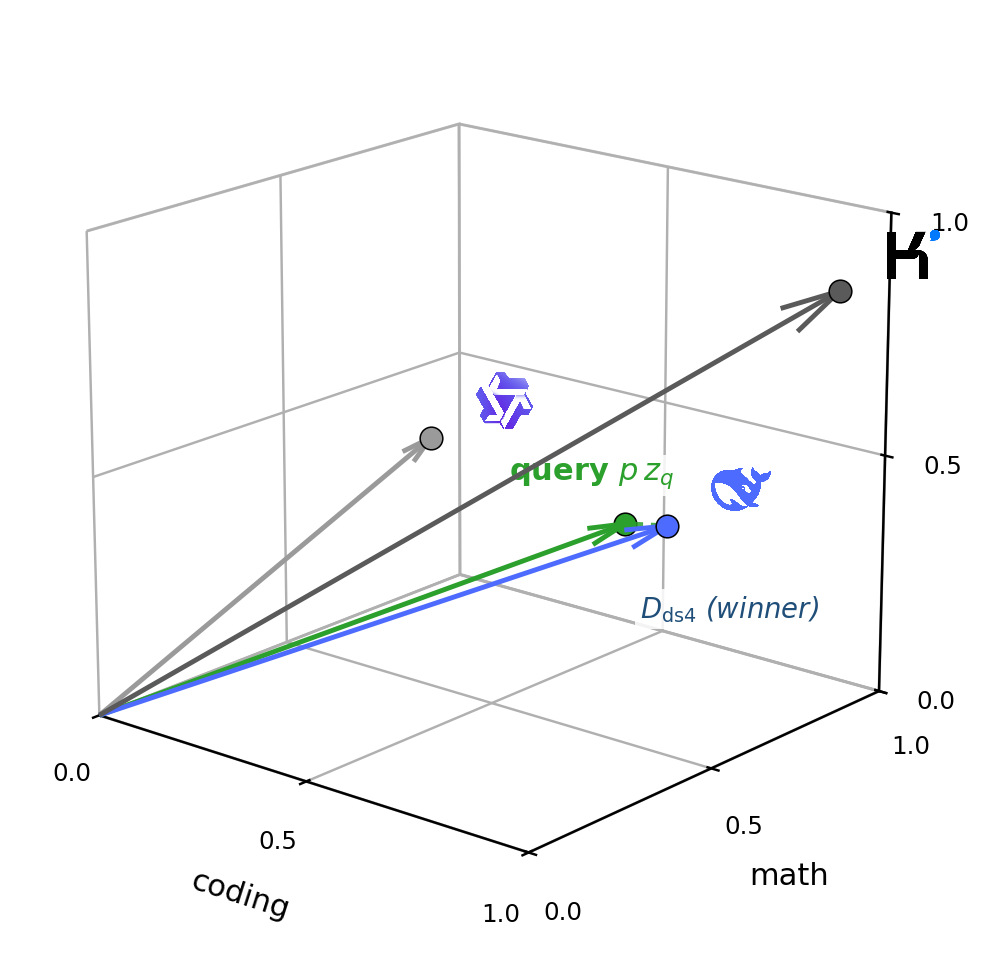
\includegraphics[width=\columnwidth]{mom_capability_3d.png}
\caption{Illustrative projection onto three of the six capability axes. The Brick router operates in the full six-dimensional capability basis; this 3D rendering is schematic. The dashed arc marks the winning distance to the selected model.}
\label{fig:mom3d}
\end{figure}

\subsection{ModernBERT capability classifier}\label{sec:brick-modernbert}
Step (iii) is a fine-tuned ModernBERT classifier~\cite{warner2024modernbert} that maps a query string to a probability vector over six capability dimensions. We fine-tune \texttt{answerdotai/ModernBERT-base} on Dataset~B, a 50k-query labeled corpus distinct from Dataset~A. Training is a W\&B~sweep over learning rate ($10^{-5}$ to $10^{-4}$, log), weight decay ($10^{-6}$ to $10^{-2}$), warmup ratio ($0.03$ to $0.12$), and number of epochs ($2$ to $5$). The winning configuration is selected by the macro-Pearson correlation on a held-out evaluation split, reaching $0.983$.
\begin{itemize}[noitemsep,topsep=2pt,leftmargin=1em]
  \item \href{https://huggingface.co/regolo/brick-modernbert-capability-classifier}{HuggingFace: regolo/brick-modernbert-capability-classifier}
  \item \href{https://wandb.ai/massa-industries/sweeps/dataset-b-modernbert/0srgzjrg}{W\&B sweep: dataset-b-modernbert / 0srgzjrg}
\end{itemize}

\begin{figure*}[!t]
\centering
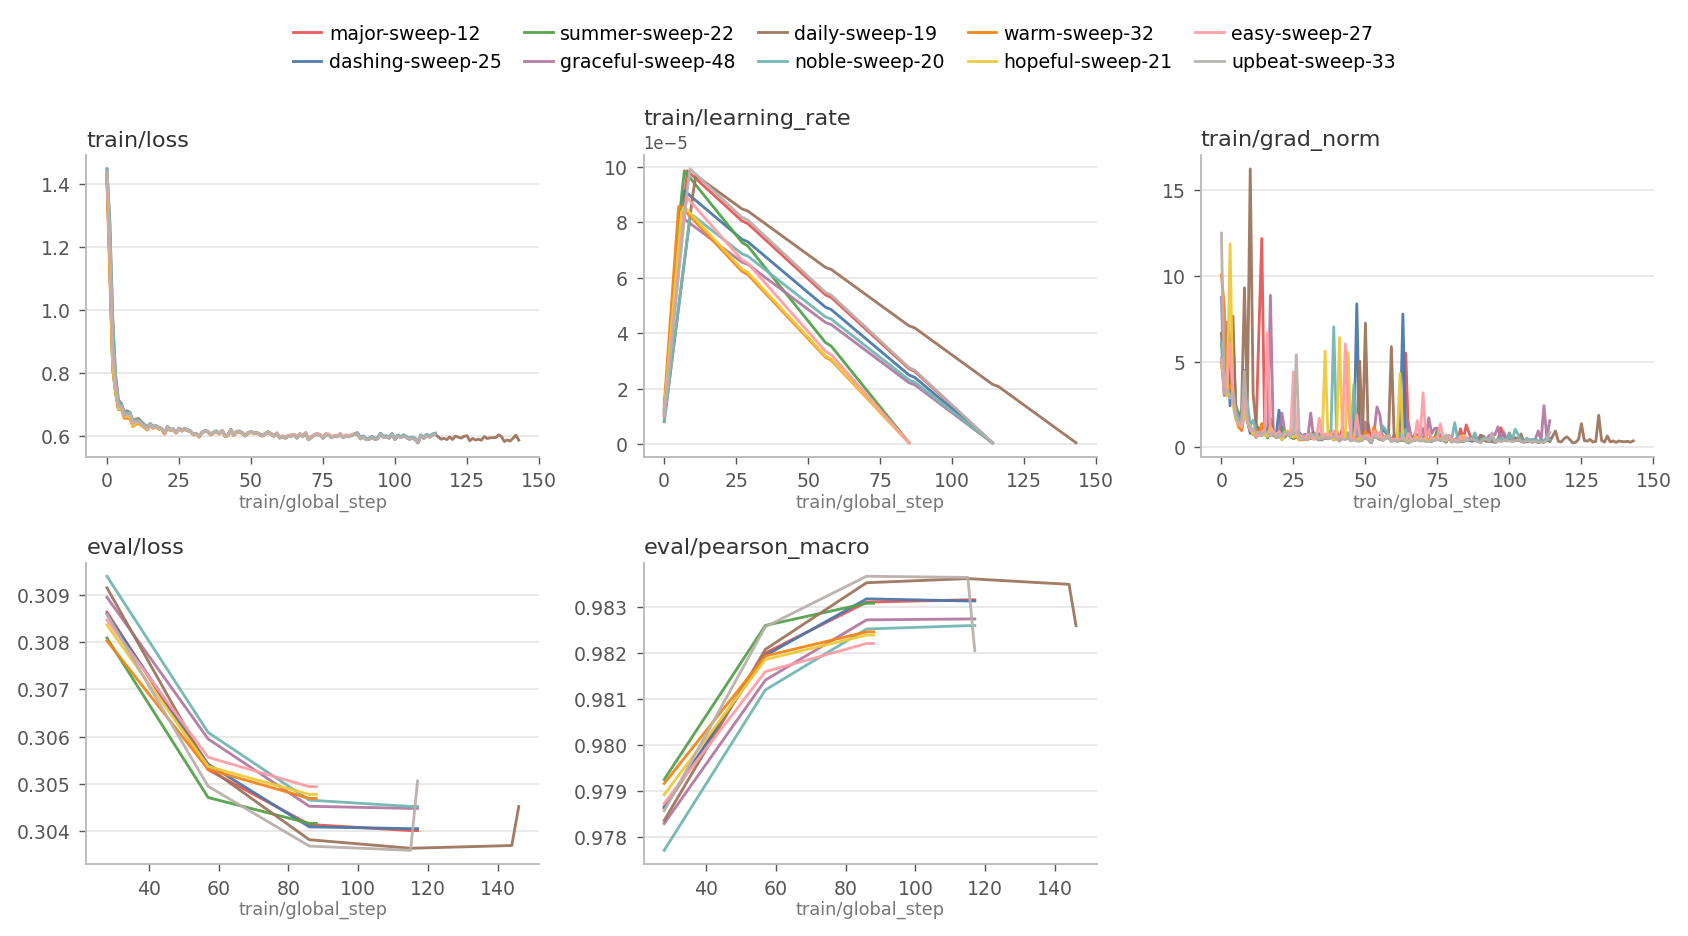
\includegraphics[width=0.98\textwidth]{modernbert_training.png}
\caption{Top-10 runs from the ModernBERT W\&B~sweep by Pearson-macro, in a multi-metric dashboard view (training loss, learning rate, gradient norm, validation loss, validation Pearson macro).}
\label{fig:modernbert}
\end{figure*}

\subsection{Complexity classifier and difficulty blending}\label{sec:brick-complexity}
Step (iv) of the pipeline is a separate fine-tuned classifier that scores how hard the query is for the pool. We use a 3-class head (\texttt{easy}/\texttt{medium}/\texttt{hard}) built on \texttt{Qwen3.5-0.8B} with LoRA adapters ($r{=}\alpha{=}32$, dropout $0.1$), fine-tuned for $3$ epochs at learning rate $10^{-4}$, batch size $16$, maximum sequence length $768$. Training uses an asymmetric over-penalty ($\lambda_{\text{over}}{=}0.7$, biasing the classifier to under- rather than over-rate difficulty) and label smoothing $0.08$; on the held-out test set ($n{=}1994$) it reaches $72.8\%$ accuracy and $0.425$ macro-F1. The classifier returns a label $\ell\in\{\text{easy},\text{medium},\text{hard}\}$ and a confidence $c\in[0,1]$.

Three anchor values bind labels to a continuous difficulty axis,
\[
  \tau_{\text{easy}}{=}0.55,\quad \tau_{\text{medium}}{=}0.72,\quad \tau_{\text{hard}}{=}0.88,
\]
and the blended difficulty $\tau_q$ consumed by the router (§\ref{sec:brick-math}) is a confidence-weighted convex combination of the predicted-label anchor and the medium anchor:
\[
  \tau_q \;=\; c\cdot\tau_{\ell} \;+\; (1-c)\cdot\tau_{\text{medium}}.
\]
When the classifier is uncertain ($c{\to}0$) the difficulty collapses to the safe medium tier ($\tau_q{\to}\tau_{\text{medium}}$); when it is confident ($c{\to}1$) it matches the predicted anchor. This blending replaces a brittle hard decision with a smooth contraction toward the centre, absorbing the residual miscalibration of the small classifier without escalating to a larger model just to break a tie. As a concrete example, the query of §\ref{sec:brick-example} is labelled \texttt{hard} with $c{=}0.51$, yielding $\tau_q = 0.51\cdot 0.88 + 0.49\cdot 0.72 = 0.802$.
\begin{itemize}[noitemsep,topsep=2pt,leftmargin=1em]
  \item \href{https://huggingface.co/regolo/brick-complexity-2-eco}{HuggingFace: regolo/brick-complexity-2-eco}
\end{itemize}

\subsection{User preference knob}\label{sec:brick-knob}
Brick exposes a continuous preference $r\in[-1,1]$ with named profiles $\mathrm{min}{\equiv}{-1}$, $\mathrm{neutral}{\equiv}0$, $\mathrm{max}{\equiv}{+1}$. The knob smoothly modulates the four routing scalars $(\mu(r),\,b(r),\,\beta(r),\,\lambda(r))$ that enter the scoring of §\ref{sec:brick-math}. Concretely, define the positive and negative branches
\[
  p^{+}(r) \;=\; \max(r,0)^{\alpha}, \qquad p^{-}(r) \;=\; \max(-r,0)^{\alpha},
\]
where $\alpha{>}0$ is a sharpness exponent (larger $\alpha$ flattens the response near $r{=}0$ and concentrates the action at the extremes). The four scalars follow a calibrated asymmetric power law:
\[
\begin{aligned}
  \mu(r)     &\;=\; \mu_0\,\exp\!\bigl(p^{+}\ln A_{\mu}^{+} \;+\; p^{-}\ln A_{\mu}^{-}\bigr), \\
  b(r)       &\;=\; b_0 \;+\; p^{+}A_{b}^{+} \;+\; p^{-}A_{b}^{-}, \\
  \beta(r)   &\;=\; \beta_0\,\exp\!\bigl(-p^{+}\ln A_{\beta}^{+} \;+\; p^{-}\ln A_{\beta}^{-}\bigr), \\
  \lambda(r) &\;=\; \lambda_0\,\exp\!\bigl(-p^{+}\ln A_{\lambda}^{+} \;+\; p^{-}\ln A_{\lambda}^{-}\bigr).
\end{aligned}
\]
The four base values $(\mu_0, b_0, \beta_0, \lambda_0)$ are the neutral-knob ($r{=}0$) defaults; the eight $A_{\cdot}^{\pm}$ are asymmetric multipliers that let calibration push harder on one side of the knob than the other. The construction is not arbitrary; below we trace where it comes from, then justify each design choice in turn.

\paragraph{Where these formulas come from.} Three constraints shape the family: continuity in $r$, identity at $r{=}0$ (neutral reproduces production defaults), and pre-calibrated targets at $r{=}\pm 1$. These constraints are met by many continuous families; we pick a one-sided power law $|r|^\alpha$ as the simplest interpretable parametrization that allows independent asymmetric calibration of the two extremes, hence $|r|^\alpha$ as the building block. Since the two extremes are not mirror images (e.g.\ $\lambda$ must shrink by ${\approx}900\times$ at $r{=}{+1}$ but inflate only ${\approx}12\times$ at $r{=}{-1}$), we split into one-sided basis functions $p^{+}(r){=}\max(r,0)^\alpha$ and $p^{-}(r){=}\max(-r,0)^\alpha$: both vanish at $0$, exactly one is unity at $\pm 1$, never overlap. The combiner is then dictated by domain: $\mu, \beta, \lambda$ must stay positive, so $x_0\cdot\exp(\cdot)$; $b$ lives in logit space, so $b_0+(\cdot)$. We wrap the calibration constants in $\ln$ inside the exponent purely for readability: at $r{=}\pm 1$ the exponent collapses to $\pm\ln A$, so $A^\pm$ is literally the multiplicative factor at each extreme (e.g.\ $A_\lambda^{+}{=}896$ reads off the table as ``$\lambda$ shrinks $896\times$ at max-quality''). The sign in front of each $p^{\pm}\ln A^{\pm}$ is fixed by routing semantics: at $r{=}{+1}$ we want $\beta, \lambda$ to shrink (minus sign) and $\mu$ to grow (plus sign); $b$ stays straight additive.

\paragraph{Why two one-sided branches $p^{+}, p^{-}$ instead of a signed $|r|^\alpha$.} A signed term would still vanish at $r{=}0$ but would force a single constant to govern both extremes. We wanted independent calibration per side because the production trade-offs are not symmetric: for example, the over-capacity penalty $\lambda$ has to deflate by a factor of about $900$ at $r{=}{+1}$ (so overkill stops mattering when the operator picks max-quality) but only needs to inflate by a factor of about $12$ at $r{=}{-1}$ (more than enough to push the router toward cheap models). That ratio of ratios cannot be expressed with a single multiplier; the split into $p^{+}, p^{-}$ with independent $A^{+}, A^{-}$ is the cheapest parametrization that buys per-side freedom while keeping continuity and intrinsic neutrality at $r{=}0$.

\paragraph{Why log-multiplicative form for $\mu, \beta, \lambda$.} These three scalars are \emph{magnitudes} that must stay strictly positive: $\mu$ scales a logit, $\beta$ scales an additive cost, $\lambda$ scales a sum of squares. Writing each one as $x_0 \cdot \exp(\dots)$ enforces positivity for free regardless of what calibration puts inside the exponent. Putting $\pm p^{\pm}\ln A$ inside, then, gives exactly $x_0 \cdot A^{\mp 1}$ at $r{=}{\pm 1}$: the constants $A^{+}$ and $A^{-}$ can then be read directly off the table as the multiplicative factors (or their inverses, depending on the sign convention) by which each scalar changes at the corresponding extreme. The calibration is interpretable by inspection.

\paragraph{Why additive form for $b$.} The bias $b$ enters the model as $z_q = b + \mu\,\mathrm{logit}(\tau_q)$, i.e. it has the dimension of a logit (real-valued, sign-bearing). Forcing positivity through $\exp$ would be wrong here; the natural choice is an additive shift, and the constants $A_b^{\pm}$ then express \emph{how many units of log-odds} the baseline moves at each extreme. For instance, $A_b^{-}{=}{-}5.87$ subtracts almost six log-odds from $b$ at $r{=}{-1}$, collapsing the requirement vector and aggressively cheapening the dispatch.

\paragraph{Why the signs on $p^{+}, p^{-}$ are inverted for $\beta, \lambda$.} By convention $r{=}{+1}$ is the max-quality profile: in that regime we want the cost coefficient $\beta$ and the over-capacity penalty $\lambda$ to be \emph{small} so the router stops worrying about price and about overkill. The negative sign in front of $p^{+}\ln A_{\beta}^{+}$ produces $\beta_0 / A_{\beta}^{+}$ at $r{=}{+1}$ (with $A_{\beta}^{+}{=}13.4$ that is $\beta \approx 0.63 / 13.4 \approx 0.047$: cost becomes nearly free, the router chases quality); the positive sign in front of $p^{-}\ln A_{\beta}^{-}$ produces $\beta_0 \cdot A_{\beta}^{-}$ at $r{=}{-1}$ (with $A_{\beta}^{-}{=}13$ that is $\beta \approx 0.63 \cdot 13 \approx 8.2$: cost dominates, the router collapses to the cheapest model). The same construction holds for $\lambda$. For $\mu$ the sign convention is the opposite: $r{=}{+1}$ should \emph{inflate} the difficulty signal so larger models qualify, hence the $+p^{+}\ln A_{\mu}^{+}$ in the exponent. The $b$ branch is simpler: $r{=}{+1}$ pushes $b$ upward by $A_b^{+}$ (queries look harder) and $r{=}{-1}$ pulls $b$ downward by $A_b^{-}$ (queries look easier).

The locked production values are listed in Table~\ref{tab:brick-knob-defaults}.

At inference, the knob is passed per-request via the HTTP header \texttt{X-Brick-Routing-Preference} (a float in $[-1,1]$) or the convenience header \texttt{X-Brick-Routing-Profile} with named values \texttt{eco}/\texttt{balanced}/\texttt{pro} mapping to $r{=}{-1},0,{+1}$. The thirteen power-law constants are loaded once from the service configuration at startup and never recomputed at routing time.

\begin{table*}[!t]
\centering
\caption{Locked production math configuration for the Brick preference knob (symbols above, values below).}
\label{tab:brick-knob-defaults}
\small
\setlength{\tabcolsep}{5pt}
\begin{tabular}{*{13}{c}}
\toprule
$\mu_0$ & $b_0$ & $\beta_0$ & $\lambda_0$ & $\alpha$ &
$A_{\mu}^{+}$ & $A_b^{+}$ & $A_{\beta}^{+}$ & $A_{\lambda}^{+}$ &
$A_{\mu}^{-}$ & $A_b^{-}$ & $A_{\beta}^{-}$ & $A_{\lambda}^{-}$ \\
\midrule
$1.07$ & $0.15$ & $0.63$ & $0.35$ & $1.56$ &
$3.24$ & $1.05$ & $13.4$ & $896$ &
$0.377$ & $-5.87$ & $13$ & $11.9$ \\
\bottomrule
\end{tabular}
\end{table*}

\subsection{Worked example}\label{sec:brick-example}
% Auto-generated by extract_example_query.py. Do not hand-edit.

\textbf{Query.} \texttt{q\_03563} (dim: \texttt{planning\_agentic}): ``Can you help me with a few tasks? First, I am playing a game where I need to calculate the evolutionary fitness of a creature. ...''

\vspace{4pt}\noindent\textbf{Step 0. Preference knob.} The caller sets $r{=}0$ (\texttt{balanced} profile), so $p^{+}{=}p^{-}{=}0$ and the four routing scalars collapse to their locked production base values (Table~\ref{tab:brick-knob-defaults}):
\[
(\mu, b, \beta, \lambda) = (\mu_0, b_0, \beta_0, \lambda_0) = (1.07, 0.15, 0.63, 0.35).
\]

\vspace{4pt}\noindent\textbf{Step 1. Capability distribution} $p(x)$ from ModernBERT (six entries, sum to one):
\vspace{-2pt}\begin{center}\small
\begin{tabular}{l r r r r r r }
\toprule
$c$ & \texttt{cod} & \texttt{crea} & \texttt{ifo} & \texttt{math} & \texttt{plan} & \texttt{wld} \\
$p_c$ & 0.09 & 0.53 & 0.09 & 0.09 & 0.09 & 0.09 \\
\bottomrule
\end{tabular}\end{center}
\vspace{-4pt}{\footnotesize\noindent(Values rounded to two decimals for display; full-precision probabilities sum to one.)}

\vspace{4pt}\noindent\textbf{Step 2. Complexity and difficulty lift.} The complexity head labels the query \texttt{hard} with confidence $0.51$, blending into $\tau_q{=}0.802$. The effective difficulty logit is
\[
z_q \;=\; b + \mu\,\mathrm{logit}(\tau_q) \;=\; 0.15 + 1.07\cdot1.401 \;=\; 1.649.
\]

\vspace{4pt}\noindent\textbf{Step 3. Per-capability requirement} $r_{q,c}{=}p_c\,z_q$ (with $z_q{=}1.649$):
\vspace{-2pt}\begin{center}\small
\begin{tabular}{l r r r r r r }
\toprule
$c$ & \texttt{cod} & \texttt{crea} & \texttt{ifo} & \texttt{math} & \texttt{plan} & \texttt{wld} \\
\midrule
$p_c$ & 0.09 & 0.53 & 0.09 & 0.09 & 0.09 & 0.09 \\
$r_{q,c}$ & 0.16 & 0.87 & 0.16 & 0.16 & 0.16 & 0.16 \\
\bottomrule
\end{tabular}\end{center}
\noindent\textbf{Step 4. Per-model capacity} $v_{m,c}{=}p_c\,\mathrm{logit}(s_{m,c})$, with $S$ the offline-calibrated skill matrix:
\vspace{-2pt}\begin{center}\scriptsize
\begin{tabular}{l r r r r r r }
\toprule
$c$ & \texttt{cod} & \texttt{crea} & \texttt{ifo} & \texttt{math} & \texttt{plan} & \texttt{wld} \\
\midrule
$s_{qwen,c}$ & 0.715 & 0.512 & 0.810 & 0.912 & 0.577 & 0.180 \\
$v_{qwen,c}$ & 0.09 & 0.02 & 0.14 & 0.22 & 0.03 & -0.14 \\
$s_{ds4,c}$ & 0.821 & 0.658 & 0.863 & 0.935 & 0.621 & 0.489 \\
$v_{ds4,c}$ & 0.14 & 0.34 & 0.17 & 0.25 & 0.05 & -0.00 \\
$s_{kimi,c}$ & 0.904 & 0.752 & 0.870 & 0.944 & 0.642 & 0.344 \\
$v_{kimi,c}$ & 0.21 & 0.58 & 0.18 & 0.27 & 0.06 & -0.06 \\
\bottomrule
\end{tabular}\end{center}
\noindent\textbf{Step 5. Asymmetric residuals.} $u_{m,c}{=}\max(0, r_{q,c}{-}v_{m,c})$ (under-capacity, model too weak), $o_{m,c}{=}\max(0, v_{m,c}{-}r_{q,c})$ (over-capacity, overkill):
\vspace{-2pt}\begin{center}\scriptsize
\begin{tabular}{l r r r r r r }
\toprule
$c$ & \texttt{cod} & \texttt{crea} & \texttt{ifo} & \texttt{math} & \texttt{plan} & \texttt{wld} \\
\midrule
$u_{qwen,c}$ & 0.07 & 0.84 & 0.02 & 0.00 & 0.13 & 0.30 \\
$o_{qwen,c}$ & 0.00 & 0.00 & 0.00 & 0.07 & 0.00 & 0.00 \\
$u_{ds4,c}$ & 0.01 & 0.52 & 0.00 & 0.00 & 0.11 & 0.16 \\
$o_{ds4,c}$ & 0.00 & 0.00 & 0.02 & 0.10 & 0.00 & 0.00 \\
$u_{kimi,c}$ & 0.00 & 0.29 & 0.00 & 0.00 & 0.10 & 0.22 \\
$o_{kimi,c}$ & 0.06 & 0.00 & 0.02 & 0.11 & 0.00 & 0.00 \\
\bottomrule
\end{tabular}\end{center}
\noindent\textbf{Step 6. Distance, cost penalty, total score.} $D_m{=}\sqrt{\sum_c(u_{m,c}^{2}+\lambda\,o_{m,c}^{2})}$ (with $\lambda{=}0.35$) and $J_m{=}D_m{+}\beta\,c_m$ (with $\beta{=}0.63$). The routing-math cost scalar $c_m$ comes from §\ref{sec:pool}; the realised per-call USD cost $a_m^{\$}$ is shown alongside for reference:
\vspace{-2pt}\begin{center}\scriptsize\setlength{\tabcolsep}{4pt}
\begin{tabular}{l r r r r r c}
\toprule
\textbf{model} & $c_m$ & $a_m^{\$}$ & $D_m$ & $\beta c_m$ & $J_m$ & \textbf{sel.} \\
\midrule
\mdlogo{qwen}\,\texttt{qwen} & 0.10 & \$0.001386 & 0.908 & 0.063 & 0.971 &  \\
\mdlogo{ds4}\,\texttt{ds4}   & 0.40 & \$0.002895 & 0.562 & 0.252 & 0.814 &  \\
\mdlogo{kimi}\,\texttt{kimi} & 0.60 & \$0.030703 & 0.380 & 0.378 & 0.758 & $\checkmark$ \\
\bottomrule
\end{tabular}\end{center}
\vspace{4pt}\noindent\textbf{Step 7. Decision.} $m^{\star}=\arg\min_m J_m = \mdlogo{kimi}\,\texttt{kimi2.6}$ ($J_{\text{qwen}}{=}0.971$, $J_{\text{ds4}}{=}0.814$, $J_{\text{kimi}}{=}0.758$). The dominant capability is \texttt{creative\_synthesis} at $p{=}0.53$, and $\tau_q{=}0.80$ inflates the per-capability requirement; the qwen capacity on that dimension falls short, so its under-capacity penalty exceeds the cost gap to kimi.


% --- Mini table 3 cherry-picked queries ---
\begin{table}[H]
\centering
\caption{Two additional Brick decisions across capability dimensions, with the dominant capability probability and complexity-derived difficulty.}
\label{tab:example_queries}
\small
\begin{tabular}{l l r l}
\toprule
\textbf{Dimension} & \textbf{Dominant cap.} & $\tau_q$ & \textbf{Selected} \\
\midrule
\texttt{coding} & \texttt{crea}{=}0.66 & 0.56 & \mdlogo{qwen}\,\texttt{qwen} \\
\texttt{planning\_agentic} & \texttt{pln}{=}0.57 & 0.72 & \mdlogo{kimi}\,\texttt{kimi} \\
\bottomrule
\end{tabular}
\end{table}


\section{Brick Results on Dataset A}\label{sec:results}
Table~\ref{tab:brick_oof} reports Brick's full-dataset out-of-fold curve under stratified $5$-fold skill-vector calibration. For each fold, skill vectors are calibrated on the four held-in folds and evaluated on the held-out fold; knob hyperparameters are fixed from prior development. This protocol uses the entire dataset while avoiding per-example leakage in the skill estimates. It should be read as an in-domain calibrated evaluation, not as a zero-shot result.

\begin{table}[H]
\centering
\caption{Brick out-of-fold results on Dataset~A under locked knob hyperparameters.}
\label{tab:brick_oof}
\small
\begin{tabular}{l r r r r}
\toprule
\textbf{Profile} & $r$ & \textbf{Sel.\,acc.} & \textbf{Avg.\,cost} & \textbf{Dist.\,(\%)} \\
\midrule
min     & $-1.0$           & $63.17\%$          & $0.100$ & $100/0/0$ \\
low     & $-0.5$           & $63.17\%$          & $0.100$ & $100/0/0$ \\
neutral & $\phantom{-}0.0$ & $68.46\%$          & $0.192$ & $71/25/3$ \\
high    & $+0.5$           & $74.18\%$          & $0.359$ & $25/59/16$ \\
max     & $+1.0$           & $\mathbf{76.98\%}$ & $0.537$ & $0/31/69$ \\
\bottomrule
\end{tabular}
\end{table}

\paragraph{Skill estimator note.} The skill matrix $S$ described in §\ref{sec:brick-math} is the production-locked, Bayesian-smoothed estimator with pseudo-count $k{=}8$. The per-fold skill vectors used to produce Table~\ref{tab:brick_oof} are computed by a different routine: a probability-weighted empirical accuracy
\[
  s_{m,c} \;=\; \mathrm{clip}\!\left(\frac{\sum_q p_c(q)\,\mathbb{I}[m\text{ correct on }q]}{\sum_q p_c(q)},\; 0.02,\; 0.98\right),
\]
with soft capability weights $p_c(q)$ from the ModernBERT classifier and a hard floor/ceiling at $[0.02, 0.98]$ in lieu of an explicit prior. The two estimators converge in the large-support limit and the choice is empirically inconsequential for the routing decision at the per-fold scale of Dataset~A.

The max-quality profile reaches $76.98\%$, exceeding always-\texttt{kimi} ($75.02\%$) by $+1.96$ pp while spending $0.537$ vs $0.600$ in normalized cost. The neutral profile sits at $68.46\%$ ($+5.29$ pp over always-\texttt{qwen}) at cost $0.192$, a roughly $5{\times}$ cheaper operating point than always-\texttt{kimi}. The gap to the $83.25\%$ oracle is the residual routing opportunity not captured by the current six-dimensional capability features and the deterministic decision rule.

\section{Latency Analysis}\label{sec:latency}
We report latency along two axes: the raw \emph{router overhead} (decision time, LLM call excluded) and the \emph{perceived end-to-end latency} (router decision plus LLM generation time).

% Auto-generated by docs/figures/aggregate_latency.py. Do not hand-edit.

\begin{table}[H]
\centering
\caption{Router decision overhead (LLM call excluded) on Dataset A ($N{=}5{,}504$). All values in milliseconds.}
\label{tab:router_overhead}
\small
\begin{tabular}{l r r r r}
\toprule
\textbf{Router} & \textbf{p50} & \textbf{p95} & \textbf{p99} & \textbf{mean} \\
\midrule
Brick (ours)            & 2998 & 3211 & 3311 & 1883 \\
Cascade Routing         & 15.1 & 19.7 & 48.6 & 16.0 \\
FrugalGPT               & 103.3 & 157.7 & 556.9 & 90.2 \\
RouteLLM binary         & 97.5 & 138.3 & 394.6 & 84.0 \\
RouteLLM tournament     & 197.8 & 306.1 & 1318 & 175.2 \\
\bottomrule
\end{tabular}
\end{table}

\begin{table}[H]
\centering
\caption{Perceived end-to-end latency (router decision plus LLM generation) on Dataset A. The MoM (Brick max profile) row joins Brick's router latency with the LLM latency of the selected model per query. Single-model baselines show LLM generation latency only.}
\label{tab:latency_perceived}
\small
\begin{tabular}{l r r r r}
\toprule
\textbf{System} & \textbf{p50} & \textbf{p95} & \textbf{p99} & \textbf{mean} \\
\midrule
always-qwen   & 21441 & 232232 & 266774 & 52677 \\
always-ds4    & 10169 & 135296 & 468067 & 41768 \\
always-kimi   & 51246 & 390276 & 738106 & 106926 \\
\textbf{Brick (MoM)}      & \textbf{22802} & \textbf{278621} & \textbf{820288} & \textbf{78178} \\
\bottomrule
\end{tabular}
\end{table}


The router-overhead numbers in Table~\ref{tab:router_overhead} reflect the Dataset~A benchmark harness, where Brick makes two auxiliary classifier calls (capability and complexity) over a remote endpoint, while Cascade Routing performs a local hash lookup. In a production deployment of Brick observed over $6{,}376$ live requests, the same decision step has a median of $494$ ms (p95 $2{,}528$ ms), reflecting warm caches and co-located classifiers. The benchmark overhead is therefore a conservative upper bound on practical decision latency.

For perceived latency (Table~\ref{tab:latency_perceived}), Brick at the max-quality profile reaches the same response-accuracy regime as always-\texttt{kimi} at less than half its median end-to-end latency ($22.8$ s vs $51.2$ s). The reason is that even at the max profile Brick routes roughly $31\%$ of queries to \texttt{deepseek-v4-flash}, which is materially faster than \texttt{kimi2.6} per generation. Figure~\ref{fig:latency_cdf} shows the latency CDFs: Brick's distribution sits to the left of always-\texttt{kimi} at every quantile, and rejoins always-\texttt{ds4} at the median.

\begin{figure}[!t]
\centering
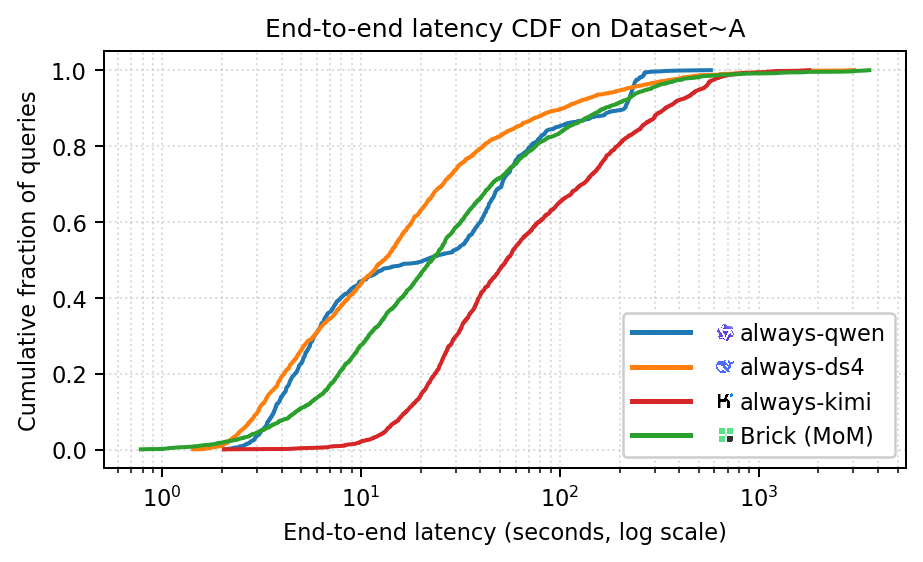
\includegraphics[width=\columnwidth]{latency_cdf.png}
\caption{End-to-end latency CDF on Dataset~A. Brick (MoM) at the max profile sits between always-\texttt{ds4} and always-\texttt{kimi}, while achieving higher response accuracy than either.}
\label{fig:latency_cdf}
\end{figure}

\section{Discussion and Limitations}\label{sec:discussion}
The reported results support three claims. (i) MoM dispatches queries across whole models and is a viable design point distinct from MoE. (ii) Within a three-model pool, a calibrated capability-aware router (Brick) exceeds the best single-model baseline on response accuracy at lower cost and lower perceived latency. (iii) The headroom above the best router and below the oracle ($83.25\%{-}76.98\%{=}6.27$ pp) reflects information the router does not yet extract from the query and the model skill matrix; this is the direction where future MoM routers will compete.

The current evaluation is in-domain calibrated: the skill matrix is fit on held-in folds of Dataset~A, and the knob hyperparameters were selected on Dataset~A. Strict external generalization should be measured on a fully out-of-distribution benchmark before claims are extended to arbitrary deployment workloads. The reported latency numbers assume a public-API deployment for the LLM call and a remote classifier endpoint for the router; numbers will move under self-hosted inference.

The MoM paradigm naturally extends to mixed open-weight and closed-weight pools. The router treats commercial APIs as additional points in the cost-capability plane. The principal open work is calibrating skill vectors for closed-weight models without leaking proprietary evaluation data and propagating their non-stationary pricing into the cost vector $a$.

\section{Conclusion}\label{sec:conclusion}
We argued that whole-model routing across heterogeneous LLM pools, framed as \emph{Mixture of Models}, is a deployment pattern worth treating as a first-class object. We instantiated it with Brick, a calibrated capability-aware router that exceeds the best single-model baseline and external routing baselines on Dataset~A, at competitive latency. We see MoM as a practical bridge for operators who want to mix open-weight and commercial closed-weight models in a single product, paying for capacity only where the query demands it.

% =============================================================================
\begin{thebibliography}{99}\small

\bibitem{hendrycks2021math}
D.~Hendrycks et al., ``Measuring Mathematical Problem Solving with the MATH Dataset,''
in \emph{Proc.\ NeurIPS Datasets and Benchmarks}, 2021.

\bibitem{cobbe2021gsm8k}
K.~Cobbe et al., ``Training Verifiers to Solve Math Word Problems,''
arXiv:2110.14168, 2021.

\bibitem{wang2024mmlupro}
Y.~Wang et al., ``MMLU-Pro: A More Robust and Challenging Multi-Task Language Understanding Benchmark,''
in \emph{Proc.\ NeurIPS Datasets and Benchmarks}, 2024.

\bibitem{zhou2023ifeval}
J.~Zhou et al., ``Instruction-Following Evaluation for Large Language Models,''
arXiv:2311.07911, 2023.

\bibitem{pyatkin2025ifbench}
V.~Pyatkin et al., ``IFBench: Granular Instruction-Following Evaluation,''
arXiv:2503.07879, 2025.

\bibitem{yan2024bfcl}
F.~Yan et al., ``Berkeley Function-Calling Leaderboard,''
Berkeley AI Research, 2024.

\bibitem{jain2024livecodebench}
N.~Jain et al., ``LiveCodeBench: Holistic and Contamination-Free Evaluation of Large Language Models for Code,''
arXiv:2403.07974, 2024.

\bibitem{wei2024simpleqa}
J.~Wei et al., ``SimpleQA: Measuring Short-Form Factuality in Large Language Models,''
arXiv:2411.04368, 2024.

\bibitem{rein2024gpqa}
D.~Rein et al., ``GPQA: A Graduate-Level Google-Proof Q\&A Benchmark,''
in \emph{Proc.\ COLM}, 2024.

\bibitem{paech2024eqbench}
S.~Paech et al., ``EQ-Bench-Creative-v3: Emotional Intelligence and Creative Writing Evaluation,'' 2024.

\bibitem{stanford2025litbench}
Stanford NLP, ``LitBench: A Literary Synthesis Benchmark for Long-Form Evaluation,'' 2025.

\bibitem{yao2024taubench}
S.~Yao et al., ``tau-bench: A Benchmark for Tool-Augmented Reasoning,''
arXiv:2406.12045, 2024.

\bibitem{ong2024routellm}
I.~Ong et al., ``RouteLLM: Learning to Route LLMs with Preference Data,''
arXiv:2406.18665, 2024.

\bibitem{chen2023frugalgpt}
L.~Chen, M.~Zaharia, and J.~Zou, ``FrugalGPT: How to Use Large Language Models While Reducing Cost and Improving Performance,''
arXiv:2305.05176, 2023.

\bibitem{jitkrittum2024cascade}
W.~Jitkrittum et al., ``Cascade Routing for Large Language Models,''
arXiv:2405.20828, 2024.

\bibitem{warner2024modernbert}
B.~Warner et al., ``Smarter, Better, Faster, Longer: A Modern Bidirectional Encoder for Fast, Memory-Efficient, and Long-Context Fine-Tuning and Inference,''
arXiv:2412.13663, 2024.

\end{thebibliography}

\end{document}
